% THIS IS SIGPROC-SP.TEX - VERSION 3.1
% WORKS WITH V3.2SP OF ACM_PROC_ARTICLE-SP.CLS
% APRIL 2009
%
% It is an example file showing how to use the 'acm_proc_article-sp.cls' V3.2SP
% LaTeX2e document class file for Conference Proceedings submissions.
% ----------------------------------------------------------------------------------------------------------------
% This .tex file (and associated .cls V3.2SP) *DOES NOT* produce:
%       1) The Permission Statement
%       2) The Conference (location) Info information
%       3) The Copyright Line with ACM data
%       4) Page numbering
% ---------------------------------------------------------------------------------------------------------------
% It is an example which *does* use the .bib file (from which the .bbl file
% is produced).
% REMEMBER HOWEVER: After having produced the .bbl file,
% and prior to final submission,
% you need to 'insert'  your .bbl file into your source .tex file so as to provide
% ONE 'self-contained' source file.
%
% Questions regarding SIGS should be sent to
% Adrienne Griscti ---> griscti@acm.org
%
% Questions/suggestions regarding the guidelines, .tex and .cls files, etc. to
% Gerald Murray ---> murray@hq.acm.org
%
% For tracking purposes - this is V3.1SP - APRIL 2009

\documentclass{acm_proc_article-sp}
\graphicspath{{./figures/}}
%\hyphenation{op-tical net-works semi-conduc-tor pre-fe-tch
%             log-struc-tured}

\usepackage{listings}
\lstset{language=C} 

\usepackage{algorithm}
\usepackage{algorithmic}


\usepackage[english]{babel}
\usepackage{blindtext}

\usepackage{etoolbox}
\makeatletter
\patchcmd{\maketitle}{\@copyrightspace}{}{}{}
\makeatother



\begin{document}

\title{Creating Patterns by Data Shuffling \\for Distributed I/O Acceleration
\titlenote{This is a project report of course CS739 Distributed System
at University of Wisconsin, Madison.}
}

%
% You need the command \numberofauthors to handle the 'placement
% and alignment' of the authors beneath the title.
%
% For aesthetic reasons, we recommend 'three authors at a time'
% i.e. three 'name/affiliation blocks' be placed beneath the title.
%
% NOTE: You are NOT restricted in how many 'rows' of
% "name/affiliations" may appear. We just ask that you restrict
% the number of 'columns' to three.
%
% Because of the available 'opening page real-estate'
% we ask you to refrain from putting more than six authors
% (two rows with three columns) beneath the article title.
% More than six makes the first-page appear very cluttered indeed.
%
% Use the \alignauthor commands to handle the names
% and affiliations for an 'aesthetic maximum' of six authors.
% Add names, affiliations, addresses for
% the seventh etc. author(s) as the argument for the
% \additionalauthors command.
% These 'additional authors' will be output/set for you
% without further effort on your part as the last section in
% the body of your article BEFORE References or any Appendices.

\numberofauthors{2} %  in this sample file, there are a *total*
% of EIGHT authors. SIX appear on the 'first-page' (for formatting
% reasons) and the remaining two appear in the \additionalauthors section.
%
\author{
\alignauthor
Jun He, Jia Xu\\
       \affaddr{Department of Computer Sciences}\\
       \affaddr{University of Wisconsin, Madison}\\
       \email{\{jhe, jiaxu\}@cs.wisc.edu}
}
% There's nothing stopping you putting the seventh, eighth, etc.
% author on the opening page (as the 'third row') but we ask,
% for aesthetic reasons that you place these 'additional authors'
% in the \additional authors block, viz.
% Just remember to make sure that the TOTAL number of authors
% is the number that will appear on the first page PLUS the
% number that will appear in the \additionalauthors section.

\maketitle
\begin{abstract}
Storage performance is critical for high
performance computer systems. PLFS (Parallel
Log-structured File System) has been developed
and it is able to speed up storage systems by
several orders of magnitudes. However, PLFS
is limited by its log, which grows to a
large size as the number of writes increases.
In this paper, We develop a system to shuffle data among distributed
processes to make data writes more regular,
which further enables PLFS's log compression
mechanism. We propose an effective and fast 
approximation scheduling algorithm to reduce 
the data movement overhead.
Our experimental results show that our 
system significantly reduces
the size of log, hence removes the
limitation of PLFS.
\end{abstract}

%\keywords{Block allocation, ext4, file system} % NOT required for Proceedings
%%%%%%%%%%%%%%%%%%%%%%%%%%%%
%%%%%%%%%%%%%%%%%%%%%%%%%%%%
%%%%%%%%%%%%%%%%%%%%%%%%%%%%
%%%%%%%%%%%%%%%%%%%%%%%%%%%%
\section{Introduction}
High performance computing is critical to scientific
discoveries. It is widely used for weather forecasting,
DNA decoding, Physics simulation, financial data processing
and so on. Usually, high performance computer systems are
equipped with high-speed and low-latency
interconnection. The compute nodes frequently exchange
data with each other. Data on one node usually has
dependency with data on another node. 

\begin{figure}[ht]
    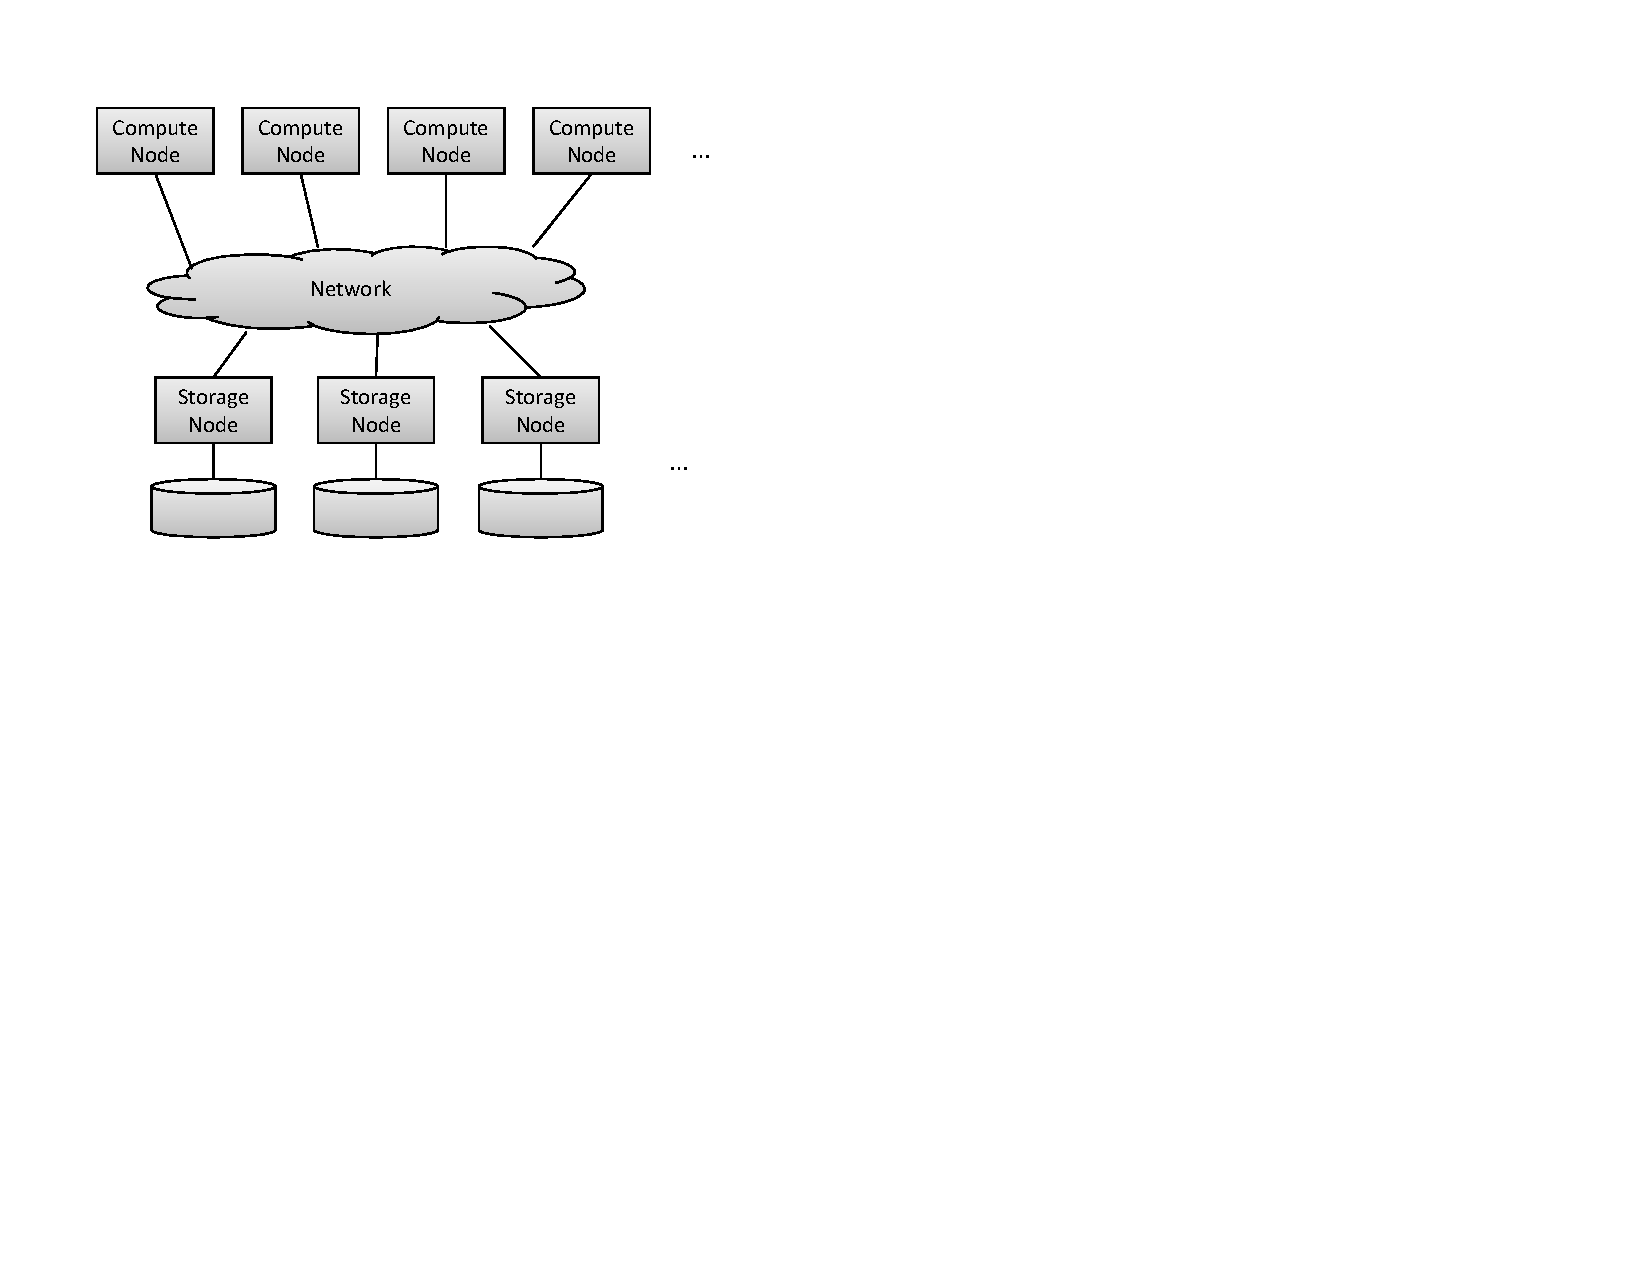
\includegraphics
    	[trim=0mm 110mm 150mm 0mm, clip, width=80mm]
    	{arch}
    \caption{An architecture of High Performance Computing system}
    \label{fig:arch}
\end{figure}


Storage system in HPC system faces great challenges.
Figure~\ref{fig:arch} shows an architecture of
HPC system. Thousands of compute nodes are connected
with each other by the high-speed network. A storage
cluster is also attached to the network. There is
a cluster file system on the storage system. The popular
choices of cluster file systems are GPFS from IBM,
Lustre from Intel (recently acquired by Intel),
PanFS from Panasas, and PVFS from Argonne 
National Laboratory. Applications like large-scale
simulations generate a great amount of data. The storage
system needs to provide TBs/sec or even PBs/sec
bandwidth to meet the requirements of the applications.
Using the storage system efficiently is hard. The
storage system performance highly depends the way the
application writes the data.

\begin{figure}[htb]
    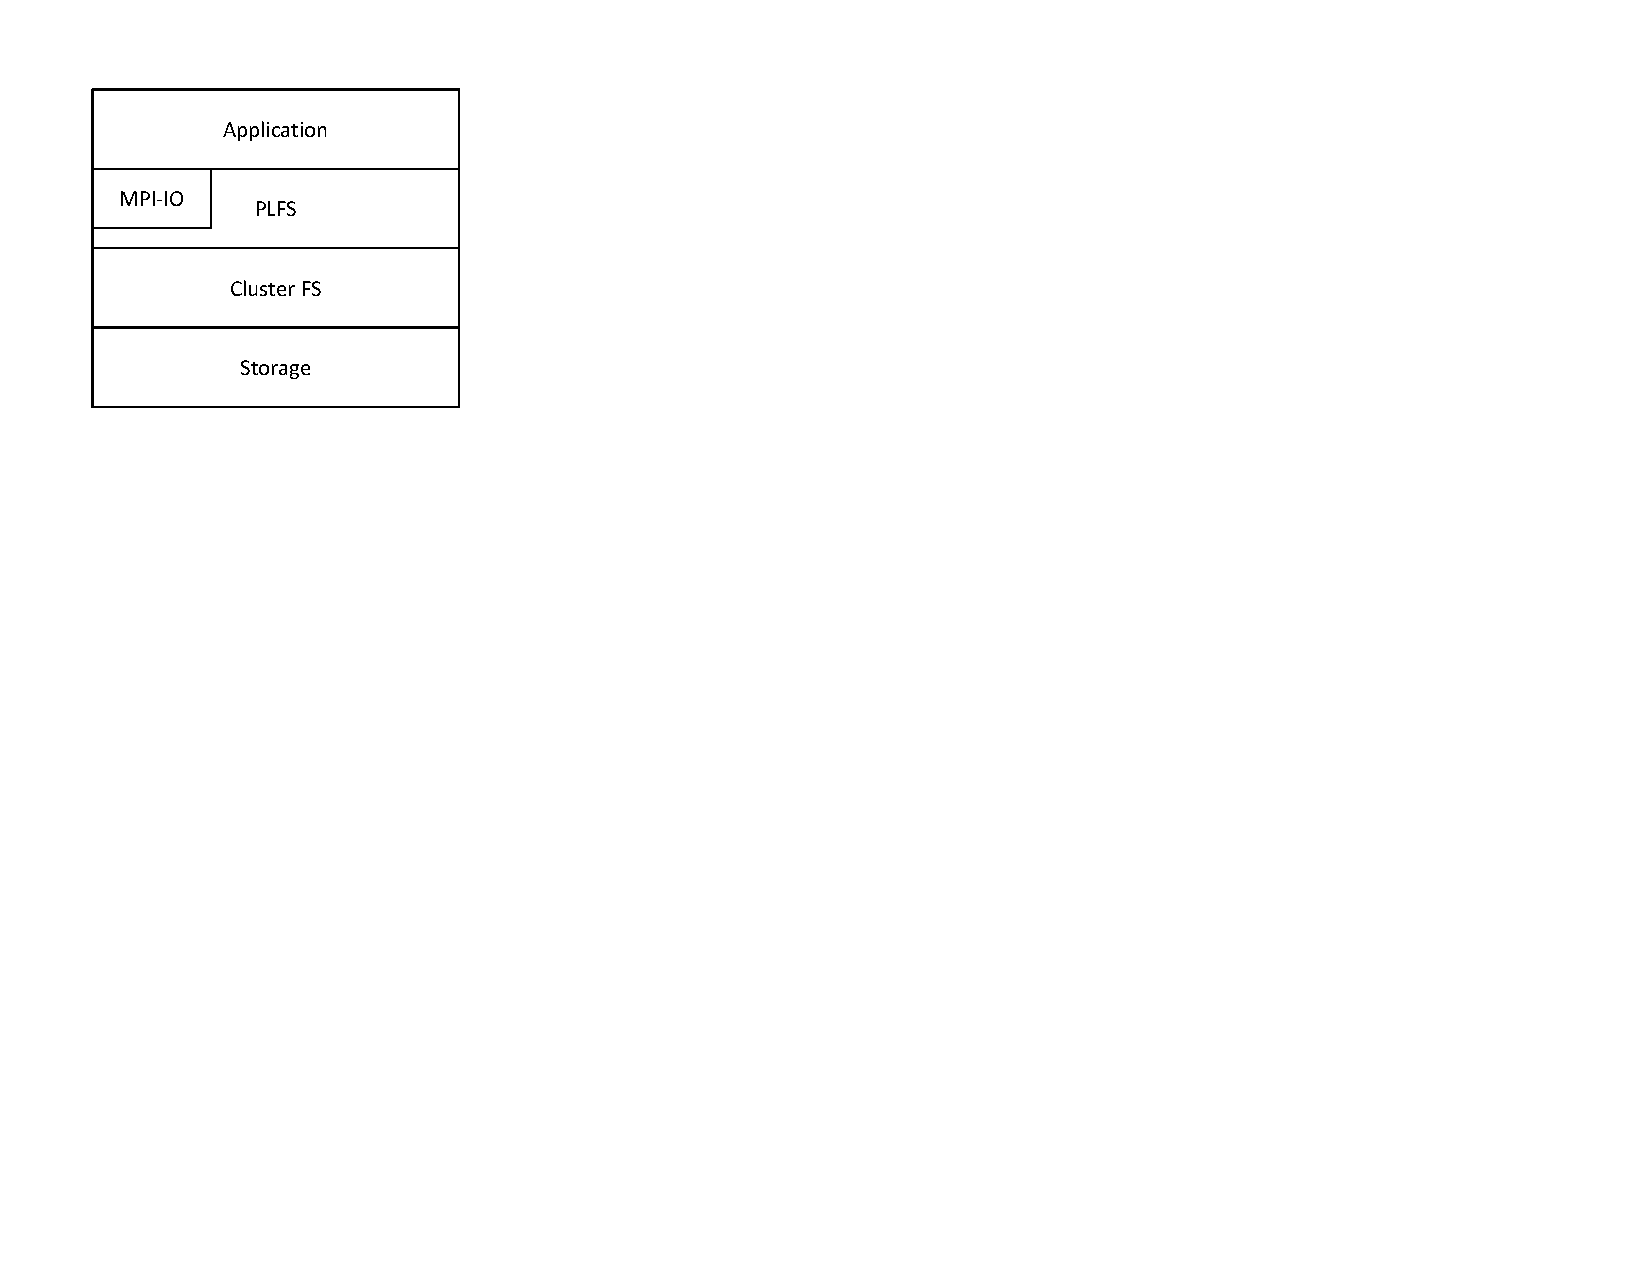
\includegraphics
    	[trim=-10mm 140mm 170mm 0mm, clip, width=80mm]
    	{layers}
    \caption{Software stack with PLFS}
    \label{fig:layers}
\end{figure}

Parallel Log-structure File System (PLFS) \cite{bent2009plfs}
has been developed
at Los Alamos National Lab to accelerate HPC storage
systems. The software stack is shown in Figure~\ref{fig:layers}.
PLFS is presented as a library. Currently, there
are three ways of using PLFS. First, the application
can directly use PLFS calls, such as plfs\_open(),
plfs\_write(), to open or write a file. 
Second, the application can use a MPI (Message Passing
Interface) library that has been linked with PLFS. 
Third, the PLFS can be mounted as a FUSE 
\footnote{FUSE stands for file system in user space. fuse.sourceforge.net}
file system.
PLFS sits on top of a `real' cluster file system.
Or we can consider PLFS as a middleware between
the application and the real cluster file system.
PLFS reorganizes the data accesses before the
data reaches the cluster file system. 
Results show that PLFS is able to speed up
the storage system by up to 150 times. 

However, PLFS has limitations. Since PLFS reorganizes
data, it needs a way to map the application's view
of the file and the physical view of the file. 
The log in PLFS serves this purpose. The log
records the information of each write the applicaion
conducts. As a result, the size of the log
is proportional to the number of writes the
application. This leads to the problem
that the large log cannot be used efficiently
or it may even crash the file system in extreme
cases. Recently, a new feature has been proposed
to PLFS so that it can compress the log if the 
writes have regular patterns\cite{HeBTGGMS13}. This works
for most of the applications. But there are
some applications that do not have regular 
write patterns or occasionally lose patterns,
in which case the pattern compression cannot
take effect. 


In order to keep a small log for PLFS even if
there is no regular write patterns, we propose
to create patterns by shuffling data.
Figure~\ref{fig:layers-shuffle} shows where
the data shuffling component resides. It resides
inside the PLFS library but above other
PLFS components. Using the data shuffling
layer, we move data from one process to another
process. The later process will write the data
on behalf of the original process. The
data movements are transparent to the rest of
PLFS. The rest of the PLFS will treat the writes
as it was coming from the application directly.
If we shuffle data in a way that the resulting
writes form a pattern, PLFS can compress the log.

\begin{figure}[ht]
    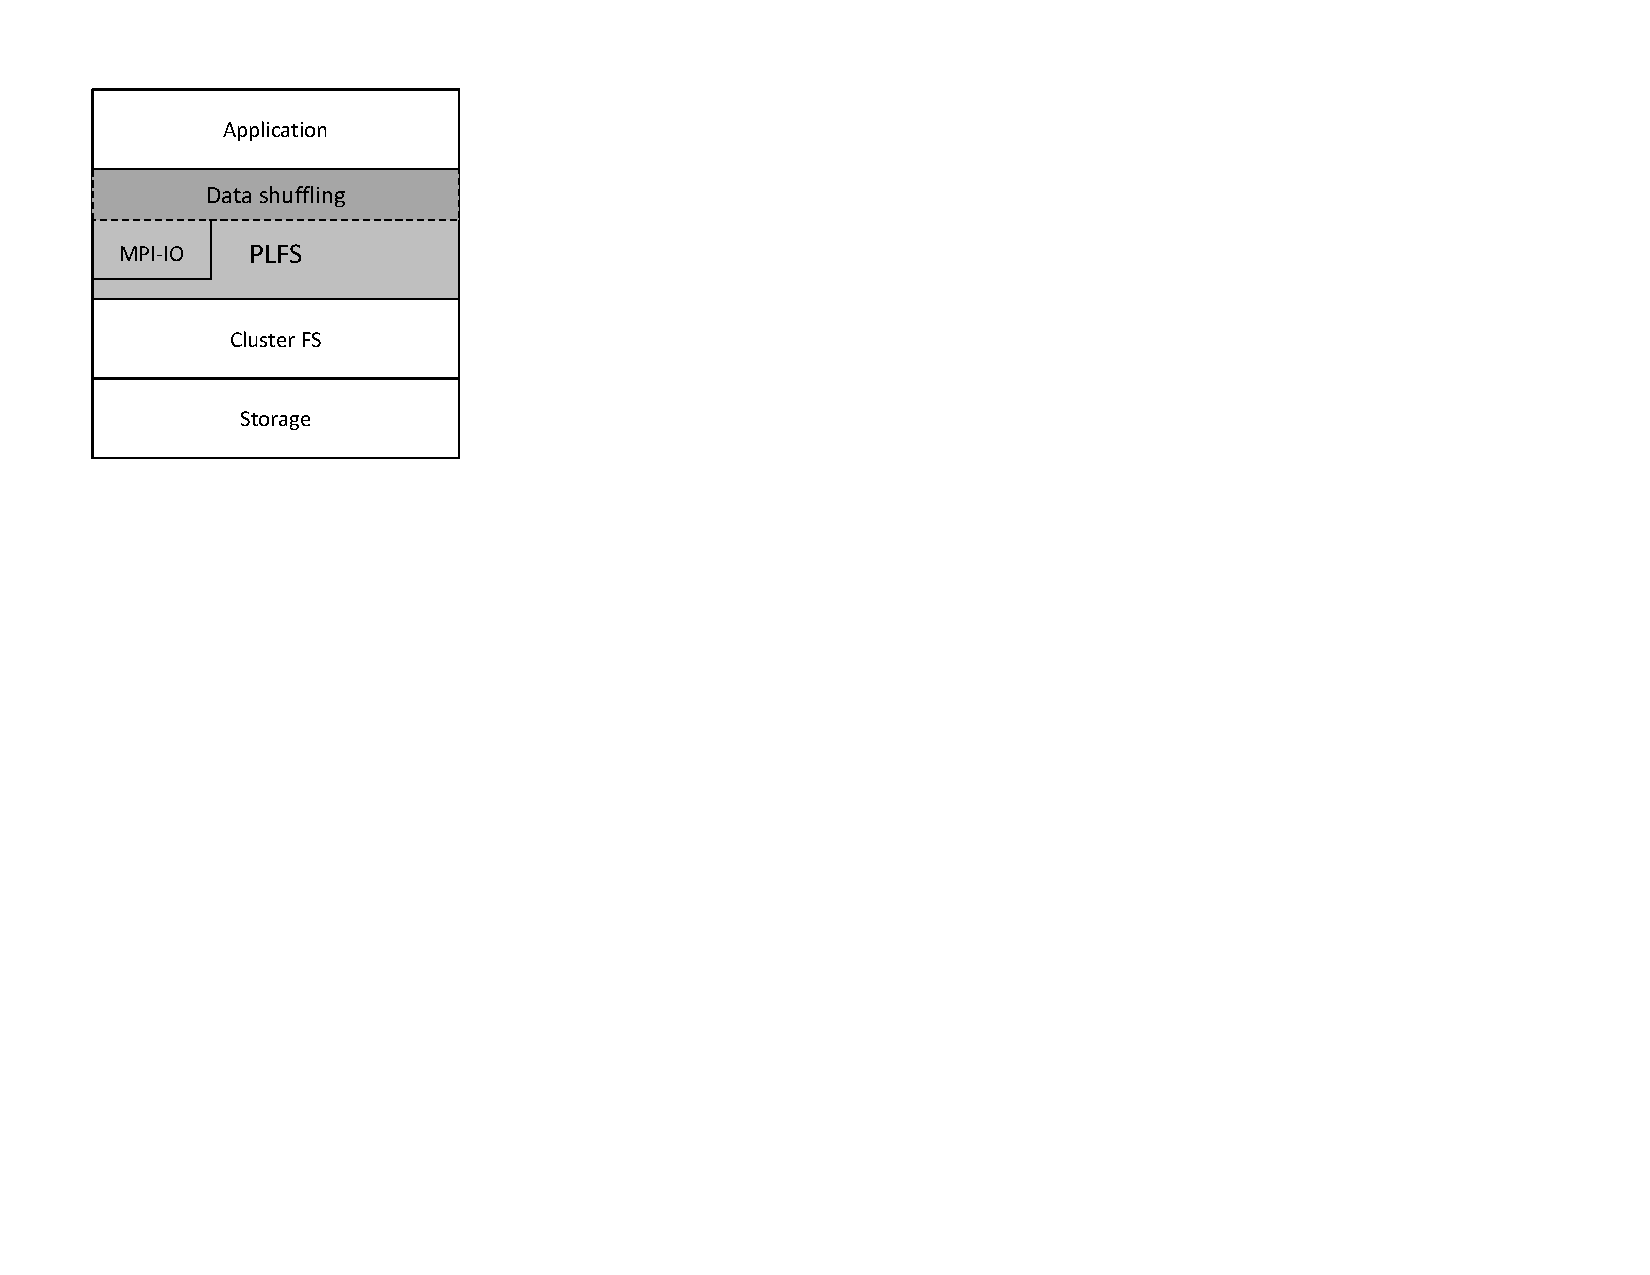
\includegraphics
    	[trim=0mm 130mm 180mm 0mm, clip, width=80mm]
    	{layers-shuffle}
    \caption{Software stack with data shuffling}
    \label{fig:layers-shuffle}
\end{figure}

Shuffling data to create regular write pattern
leads to additional data movements across
the network. Scheduling of data movements 
is essential for
the proposed idea to work efficiently.
The order for each process to send/receive
data needs to be carefully calculated
so that we can have as many concurrent
data movements between processes as possible.
In this project, we propose an approach 
to schedule the data movement activities
to reduce data movement time.

This report is organized as follows.
We describes the background
of PLFS in section~\ref{sec:plfs-background}.
In section~\ref{sec:creating-pattern},
we describe how to create pattern by data
shuffling.
In section~\ref{sec:scheduling-data-movements}
we describe how to carefully schedule data
movements to reduce data shuffling overhead.
The implementation details are in section~\ref{sec:implementation}.
Future work is in section~\ref{sec:future-work}.
Section~\ref{sec:conclusions} concludes the paper.


%%%%%%%%%%%%%%%%%%%%%%%%%%%%
%%%%%%%%%%%%%%%%%%%%%%%%%%%%
%%%%%%%%%%%%%%%%%%%%%%%%%%%%
%%%%%%%%%%%%%%%%%%%%%%%%%%%%
\section{PLFS background}
\label{sec:plfs-background}
In HPC environment, many processes run concurrently.
There are several ways for them to write data to
file. One is called \emph{N-1}. It means N processes
write to one file concurrently.
Another is called \emph{N-N}, which means N processes
write to N files. 

Generally, N-1 write is slower than N-N write. 
That is because, in file systems with locks, with
N-1 writes, when
one process is writing a segment of data, other
processes cannot write it. This serializes the
writes to that segment. With N-N write, this is 
not a problem because each process writes
its own file. Nobody contends for data. 
Due to reasons like this, N-1 write can
be orders of magnitude slower than N-N write.
Although N-1 write is slower than N-N, users
like to use N-1 write. Having only one file
is easier for their data management. 

\begin{figure}[ht]
    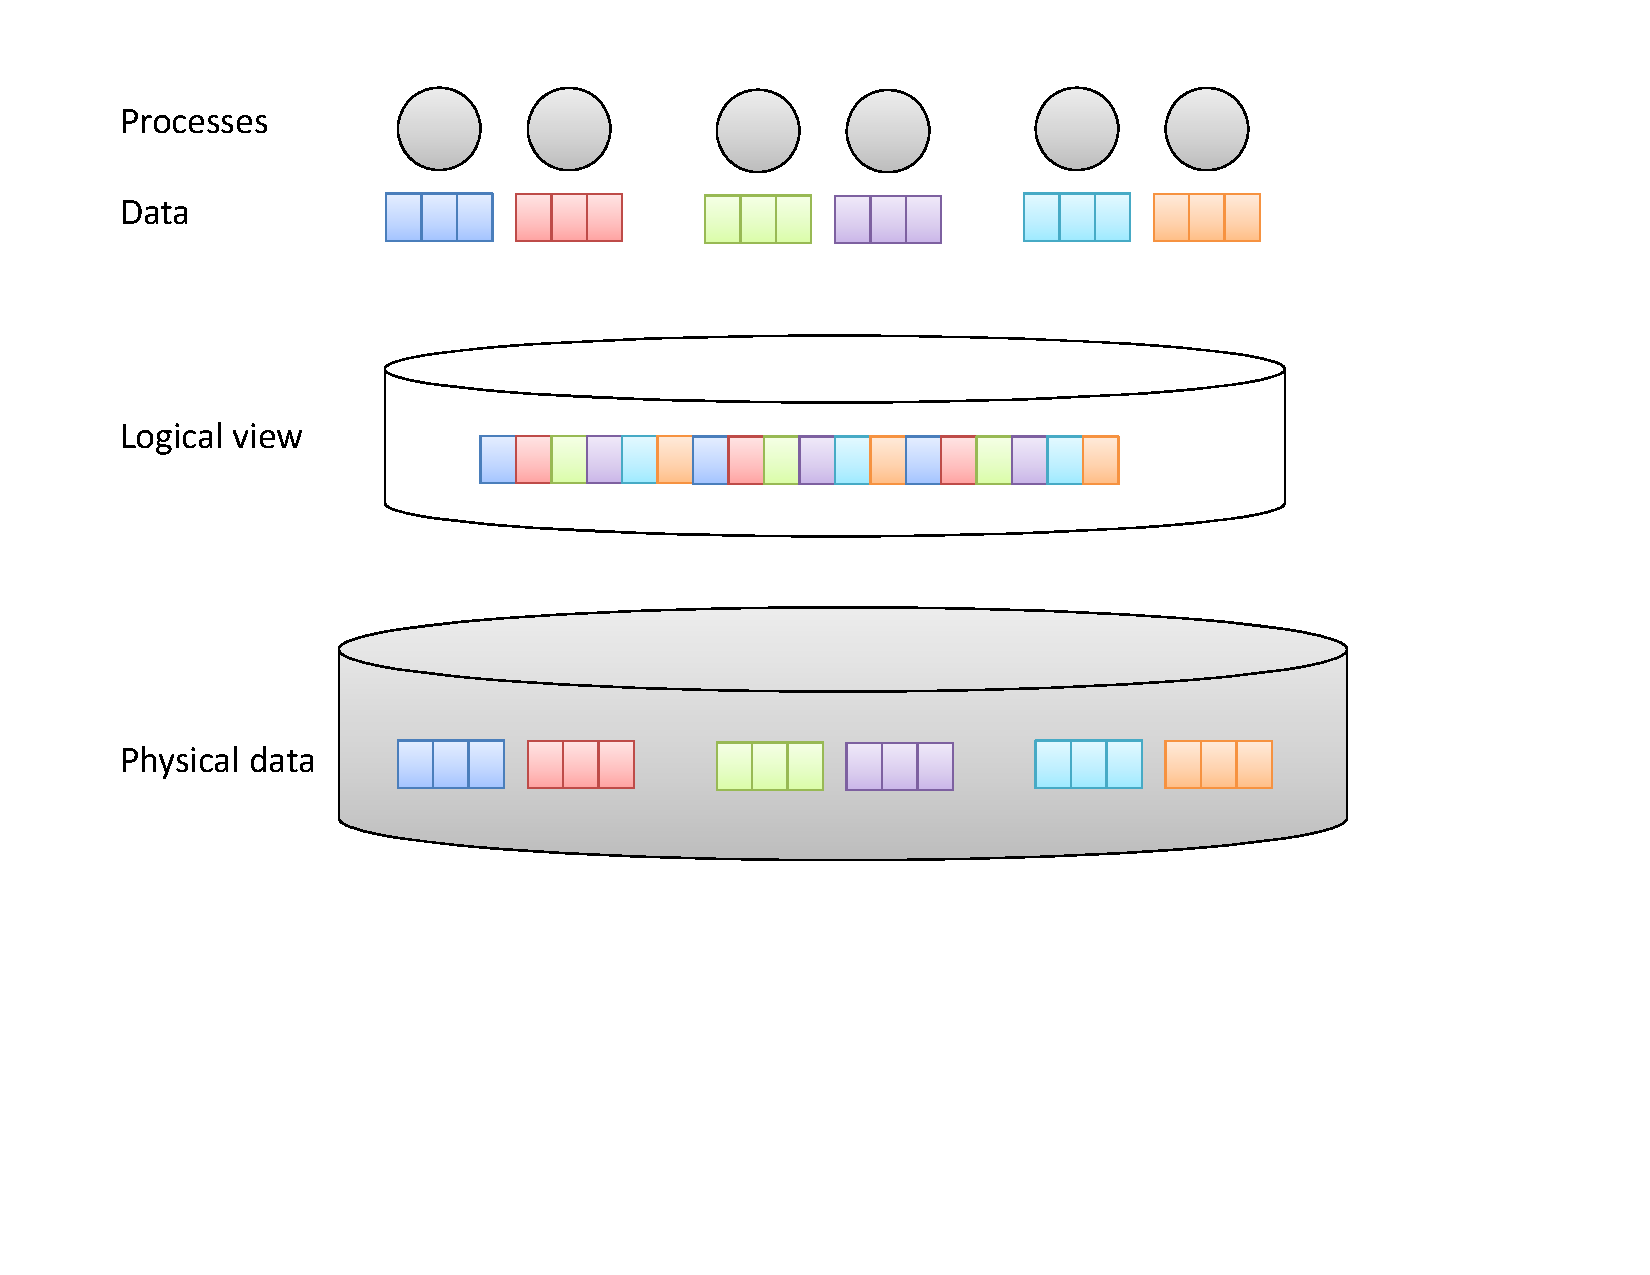
\includegraphics
    	[trim=10mm 50mm 50mm 0mm, clip, width=80mm]
    	{plfs-logical-physical}
    \caption{PLFS transparently transfers N-1 write to N-N write.}
    \label{fig:plfs-logical-physical}
\end{figure}

PLFS has been developed to mitigate this issue
by transparently transferring N-1 writes to N-N
write. Figure~\ref{fig:plfs-logical-physical}
shows how it works. From the application's
perspective, the data is the same as it were
without PLFS. The PLFS provides this illusion
to application so the application can work 
without modification. However, internally,
PLFS reorganizes data so that there are
one physical file for each process. For example,
if there are 6 processes writing to one file
called \emph{fileshared}. The application
sees only one file in PLFS. But PLFS actually
stores 6 data files in the underlying
cluster file system. 

\begin{figure}[ht]
    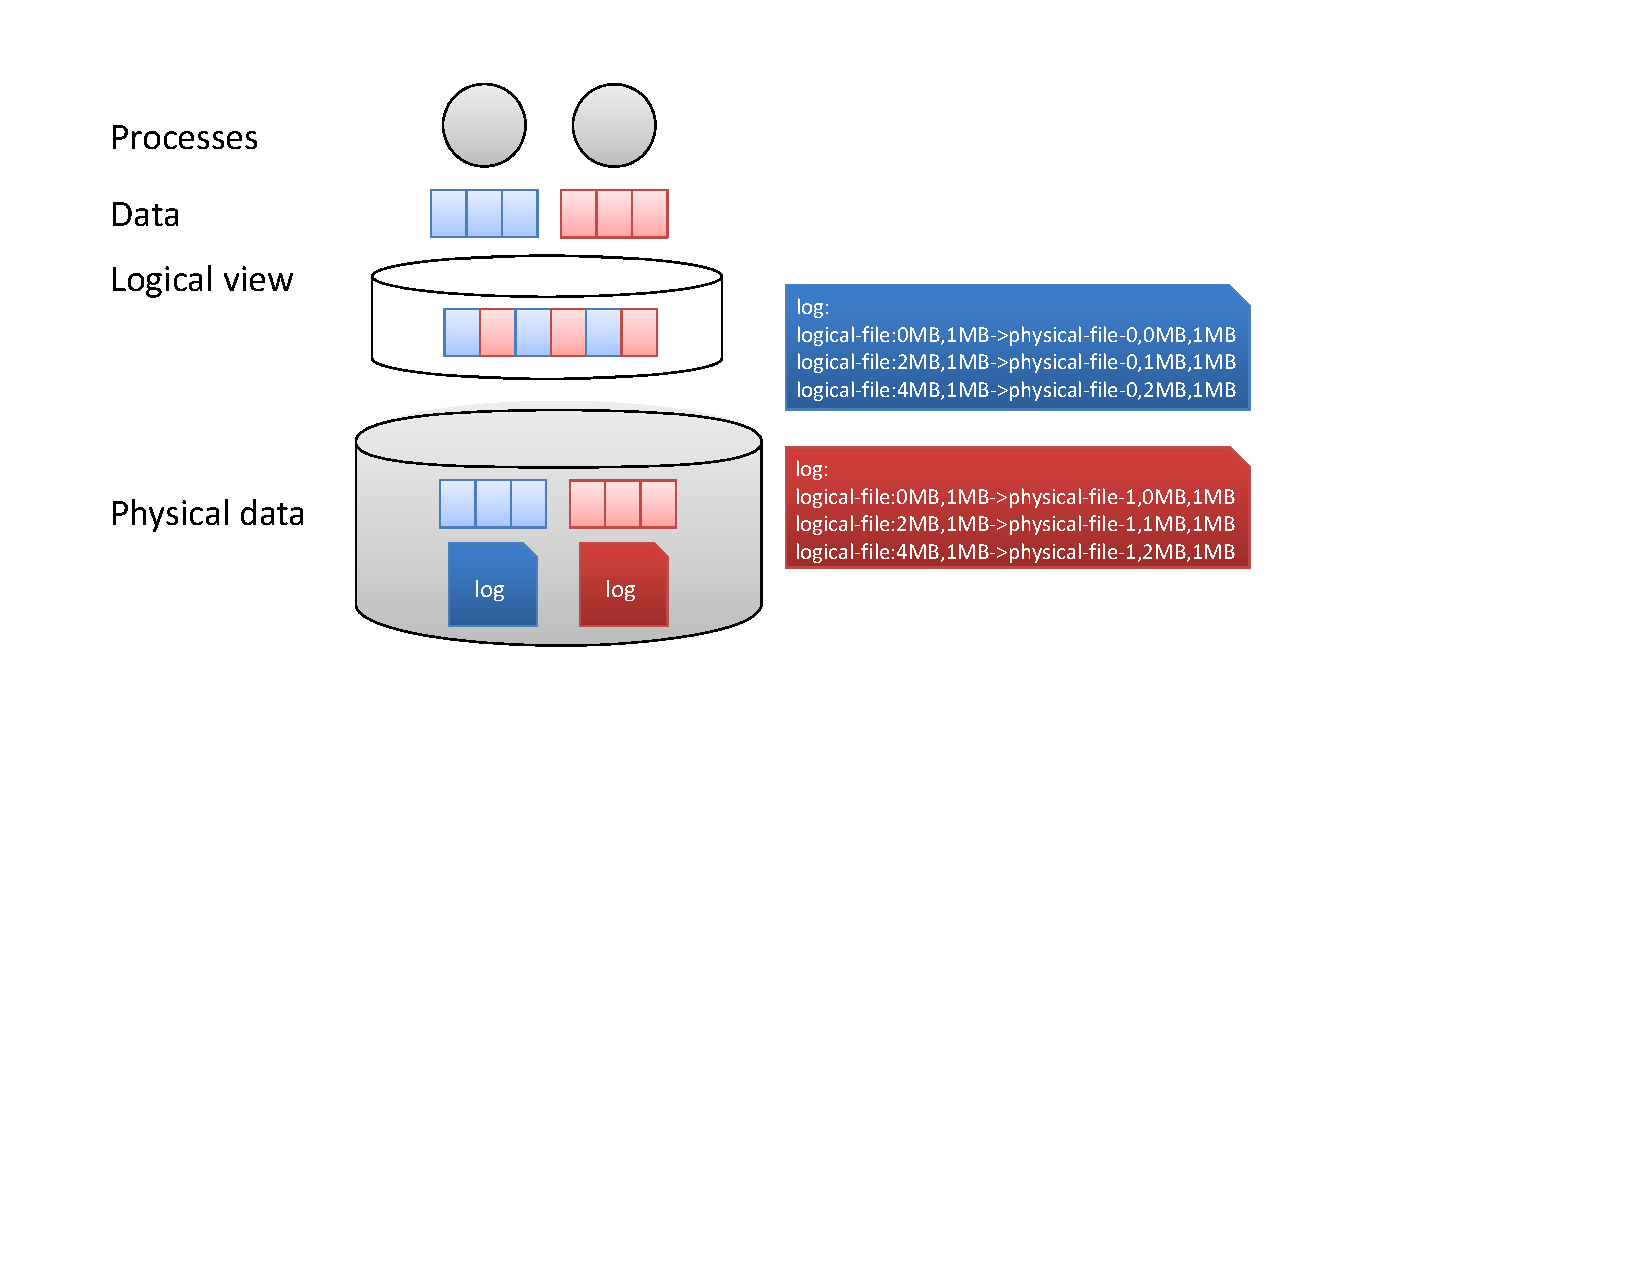
\includegraphics
    	[trim=15mm 100mm 60mm 0mm, clip, width=80mm]
    	{logexample}
    \caption{An example of log}
    \label{fig:logexample}
\end{figure}

Since the data is reorganized, we need to way
to map the application's view of the file and
the actual physical data. This is where the log
comes to help. For example, if there are
two processes writing to the same file on PLFS,
in the way shown in Figure~\ref{fig:logexample},
there will be two types of files in the
underlying cluster file system. There will
be two data files, storing data from the processes,
and two more log files, storing the mapping
information. As shown in the figure, there
are one-to-one mapping from the logical view
to the physical data. When the application reads
the logical file, PLFS will read the logs first
to build the mapping in memory. Later, when
the application reads some specific data, PLFS
looks up the physical location of the data in the
mapping table. Finally, PLFS will go to the physical
location to get the data. 

%%%%%%%%%%%%%%%%%%%%%%%%%%%%
%%%%%%%%%%%%%%%%%%%%%%%%%%%%
%%%%%%%%%%%%%%%%%%%%%%%%%%%%
%%%%%%%%%%%%%%%%%%%%%%%%%%%%
\section{Creating pattern}
\label{sec:creating-pattern}
\subsection{The pattern detection optimization}
PLFS compresses log by detecting write patterns.
This works because in practices, many of the
HPC applications present write patterns. 
The pattern here means the both the write offsets
and lengths are regular. For example, the following
code has a write pattern.

write(0, 1);\\
write(8, 1);\\
write(16, 1);\\
write(24, 1);\\

The following code has a more complicated write
pattern:

write(0, 1);\\
write(3, 1);\\
write(8, 1);\\
write(11, 1);\\
write(16, 1);\\
write(19, 1);\\
write(24, 1);\\
write(27, 1);\\

There are many applications that has write patterns.
The MILC code is a set of applications
for quantum chromodynamics. There are three write
modes in the MILC code. All of them present
regular write patterns. The FLASH code also
present write patterns. Specifically, the FLASH
code writes a file header without pattern but it
writes the rest of the file with pattern. 
There are also three anonymous applications
from Los Alamos National Lab that have write
patterns. 


There are two kinds of patterns. One is local pattern.
One is global. Local pattern means a single process's
offset-length pairs have pattern. Global
pattern means the offset-length pairs from all processes
can form a pattern. With the proposed pattern-detection
feature, PLFS can detect this kind of patterns.

\subsection{Problem of irregular writes}
Unfortunately, there are some applications that do
not have patterns. For example, an LANL application 
has three write mode. One mode writes a part of
the file without pattern. This part of the file
is illustrated in Figure~\ref{fig:lanl2pattern}.
Each color bulk represents the size of the hole
between data. Therefore, different color indicate
different hole sizes. 
Each row in the figure
shows the holes written by a process. 
The X axis is the offset of the file.
Hole size is a good 
indicator of patterns. For simplicity, 
we can think that ``places with the same color
has have the same pattern". So, we can see
that, initially, the writes have patterns (the green
part). But later, the `second column' becomes
colorful, indicating different hole sizes. This 
means they are irregular writes. In the `middle
columns', the pink bulks indicate good patterns.
Later, the writes become irregular again.
Finally, they go back to green. 

\begin{figure}[ht]
    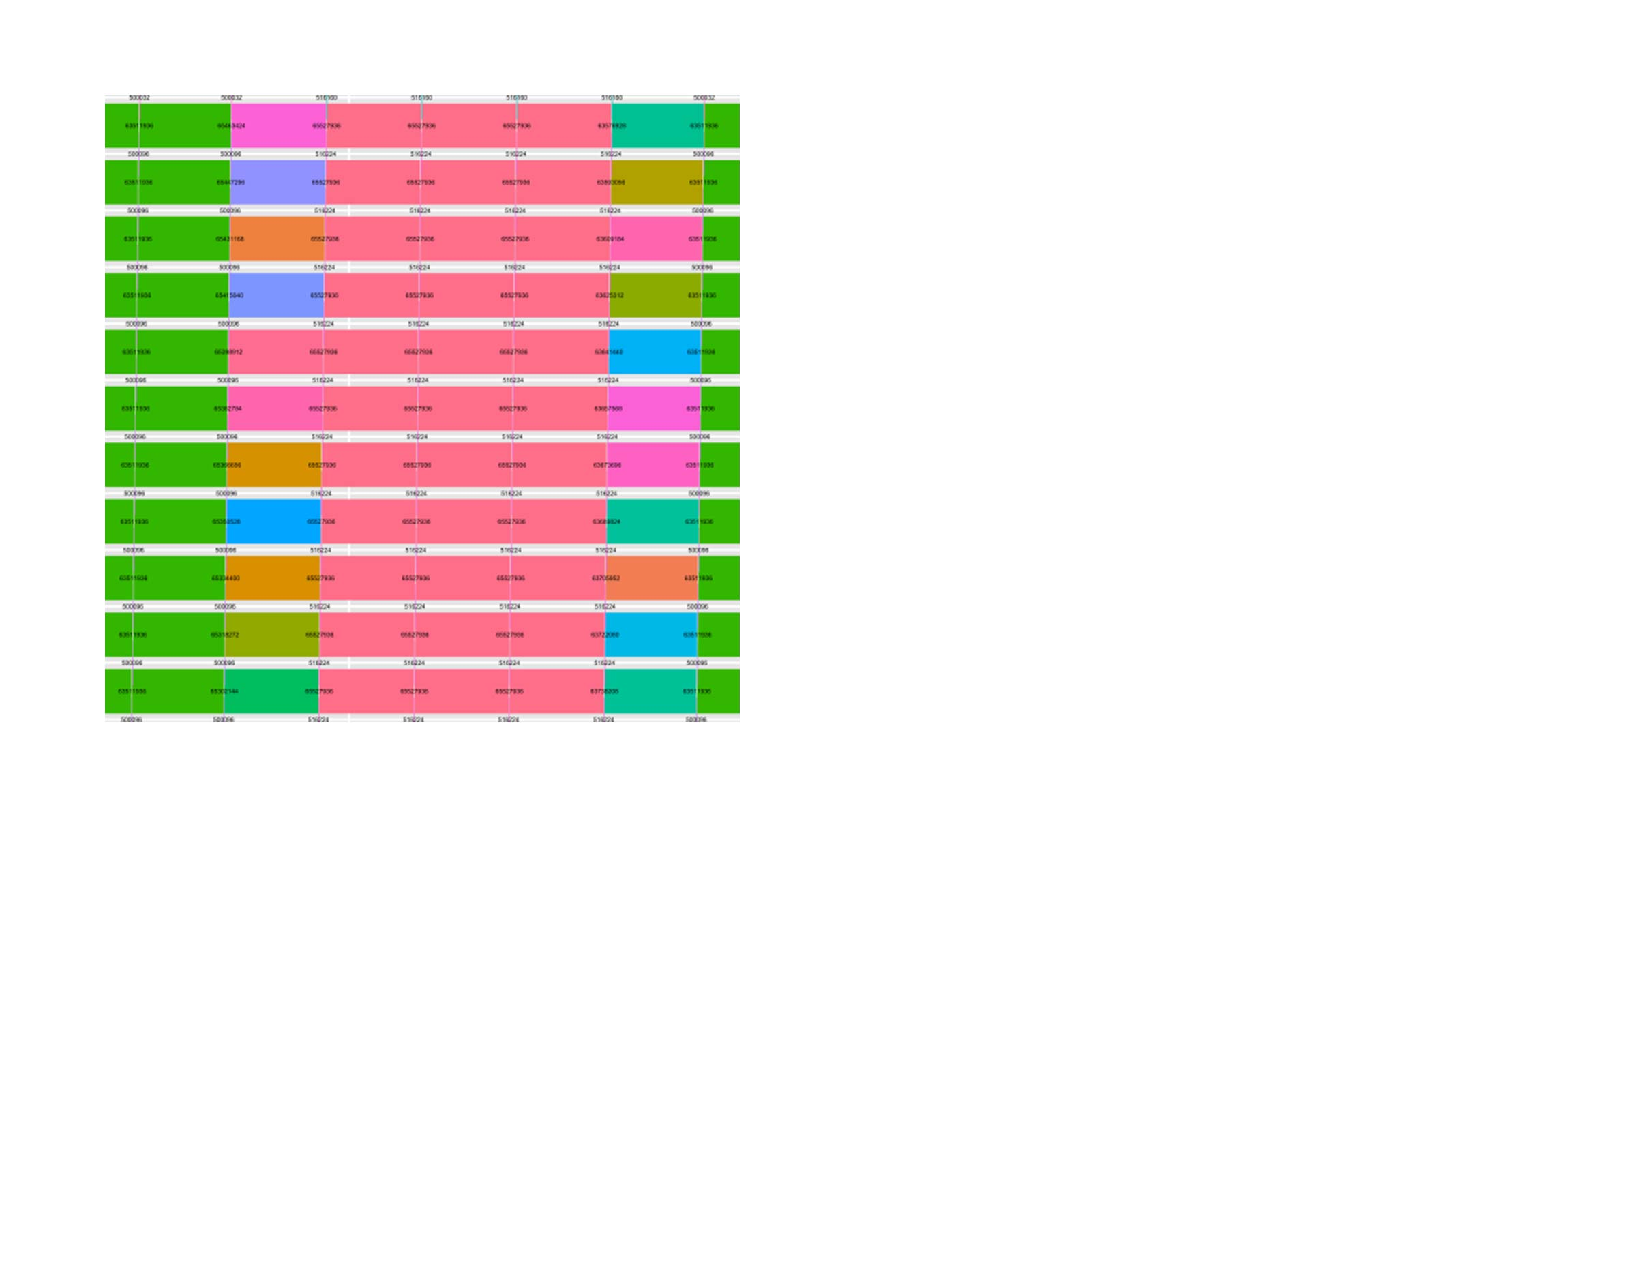
\includegraphics
    	[trim=0mm 90mm 130mm 0mm, clip, width=80mm]
    	{lanl2pattern}
    \caption{Irregular writes of LANL application 2.}
    \label{fig:lanl2pattern}
\end{figure}

This kind of irregular writes disables
the log compression in PLFS because it relies
on patterns. As a consequence, the size of
the log grows. 

\subsection{Shuffling data to create patterns}
If we can convert the irregular writes to regular
writes, we will be able to enable log compression
again. This can be done by moving (shuffling)
data between processes before the pattern detection
happens. Basically, we insert a new layer
between the application and the PLFS pattern
detection. The application will write to
this layer without any modification. 
The PLFS pattern detector will work as if
the writes are from the application directly. 

\begin{figure}[ht]
    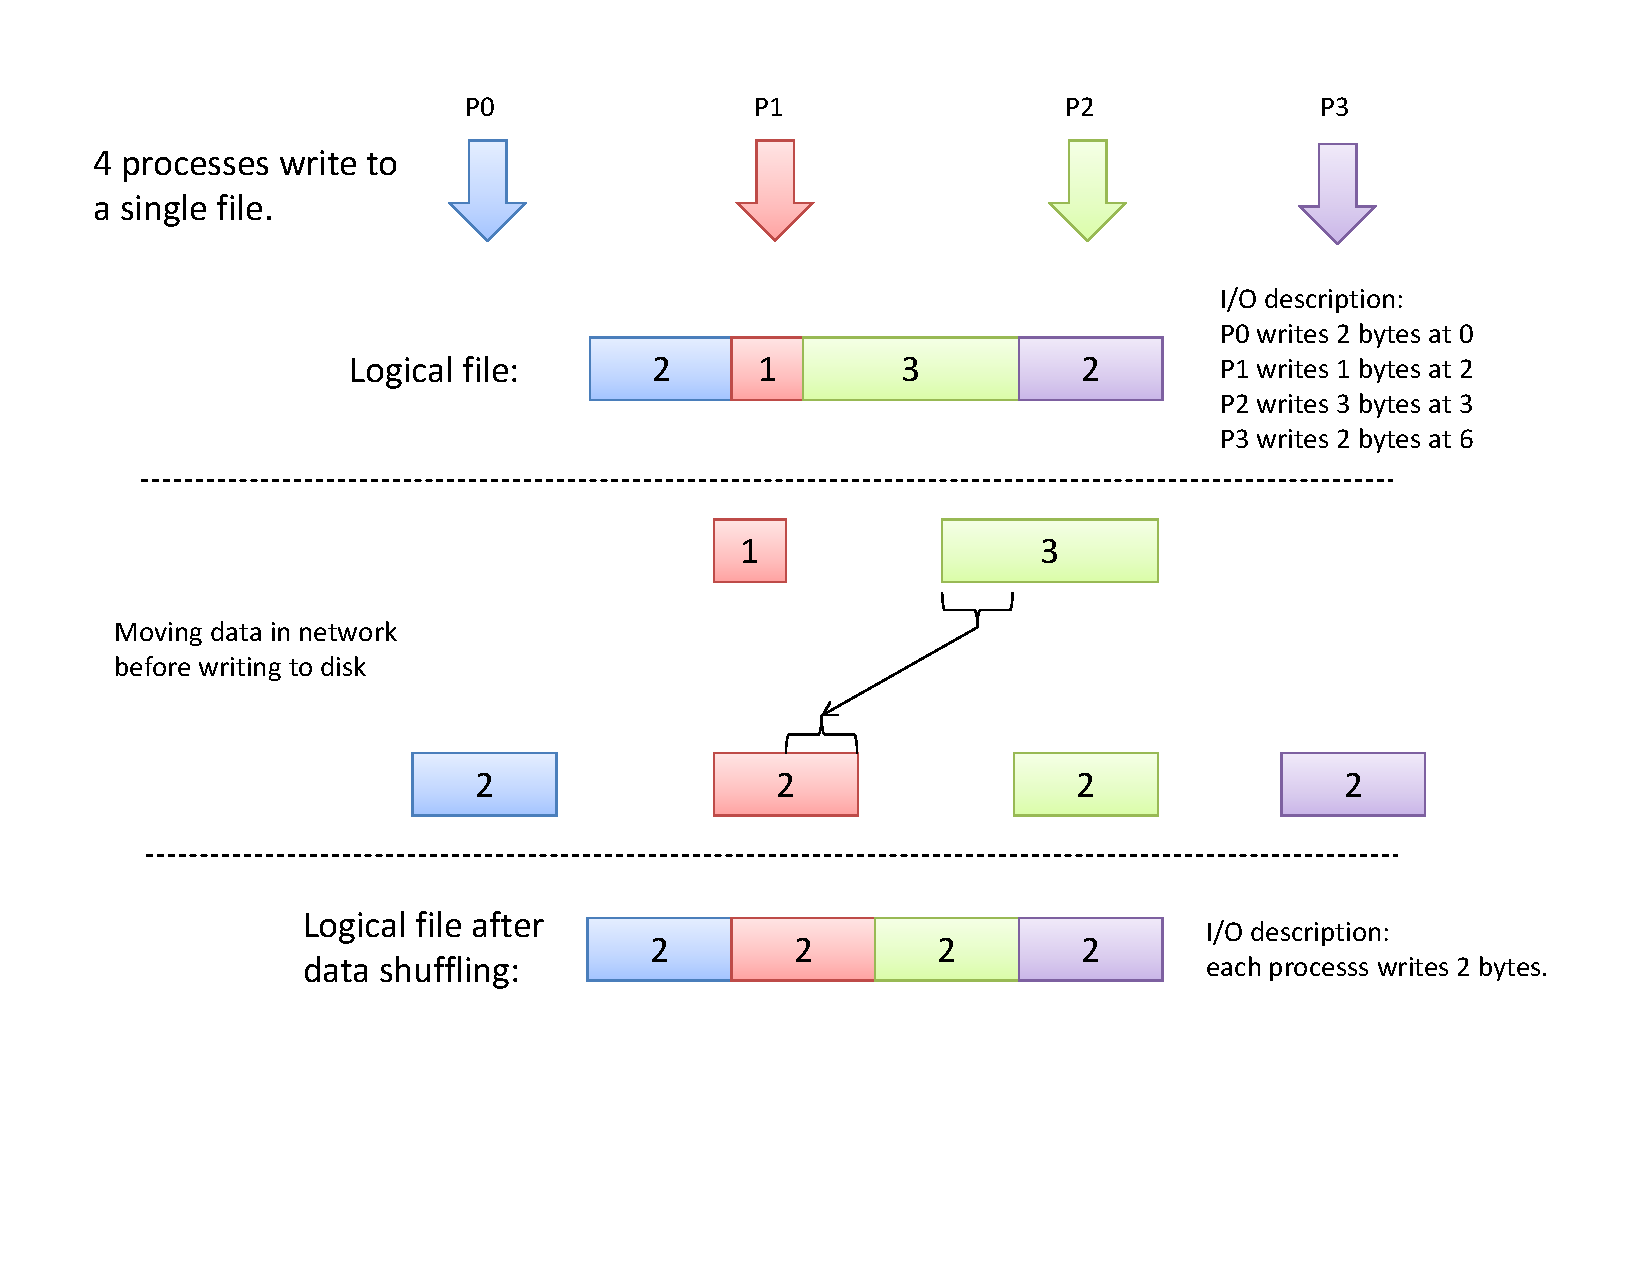
\includegraphics
    	[trim=10mm 30mm 30mm 0mm, clip, width=80mm]
    	{data-shuffling-example}
    \caption{Data shuffling example.}
    \label{fig:data-shuffling-example}
\end{figure}

As shown in Figure~\ref{fig:data-shuffling-example},
the application has four processes writing to 
the same file. They do not have an obvious regular
pattern. In order to create a regular pattern,
we move 1 byte from P2 to P1. After the movement, 
each process will have 2 bytes to write. In this
case, PLFS will be able to detect the pattern
and compress the log to a minimum size.

Currently, we create the simplest pattern.
That means we create a pattern in which
each process write $TotalBytes/$ $NumberOfProcesses$ bytes.
In other words, there will be $n$ segments,
where n is the number of processes. 
The size of a segment is $TotalBytes/NumberOfProcesses$.
Apparently, this might not be the best pattern to make.
A good pattern is a pattern that requires
the minimum amount of data movements, in terms
of the size of data to be moved and the number
of movements. There are patterns that 
PLFS can detect and require minimum amount
of movements.

A brutal force solution of finding the best
pattern to create is to try different patterns
that can be detected by PLFS on a model.
The model has two inputs. One is the current
writes. One is the writes with the pattern
to be created. By this model, we can easily
find out how much data has to be moved.
Given that
there can be an infinite number of patterns
meet this requirement, we need to limit
the number of tries we want to make. It
can be limited by a upper bound number, or 
a timeout. We pick the pattern that will
lead to the least amount of data movement.

A smarter approach would start from
the current writes. By analyzing the 
current writes, we want to find a pattern
that is very `close' to the current writes.
The `close' here means that by shifting
a very small number of data, we get a 
regular pattern. An analogy of this is
the real-world decoration pattern. If
we look at it from a long distance, 
a small variation of the pattern
cannot be seen. But if we look closely,
the small variation may bother us
and we may not consider it as regular 
pattern. A potential approach to 
find a close pattern of the writes
is by techniques in digital signal processing (DSP).
The offsets and lengths of writes are 
considered as signals.
The subtle shift is considered as noise.
The objective is to `smooth' the signal
so we can find a target regular pattern.

In practice, the brutal force approach
may be enough. Because we observed that 
most HPC applications do segmented writes
- several processes write a part of a big
file. The size of each write is usually
the same. If there are more complicated
cases, the DSP approach may help. 
Since in this project we only try to build
a working prototype for future development,
we do not focus on finding the best pattern
to be created. However, we admit this is
a very important issue in designing such a
system. We keep this as future work.


%%%%%%%%%%%%%%%%%%%%%%%%%%%%
%%%%%%%%%%%%%%%%%%%%%%%%%%%%
%%%%%%%%%%%%%%%%%%%%%%%%%%%%
%%%%%%%%%%%%%%%%%%%%%%%%%%%%
\section{Scheduling data movements}
\label{sec:scheduling-data-movements}
%% scheduling

\begin{figure}[thb]
\begin{center}
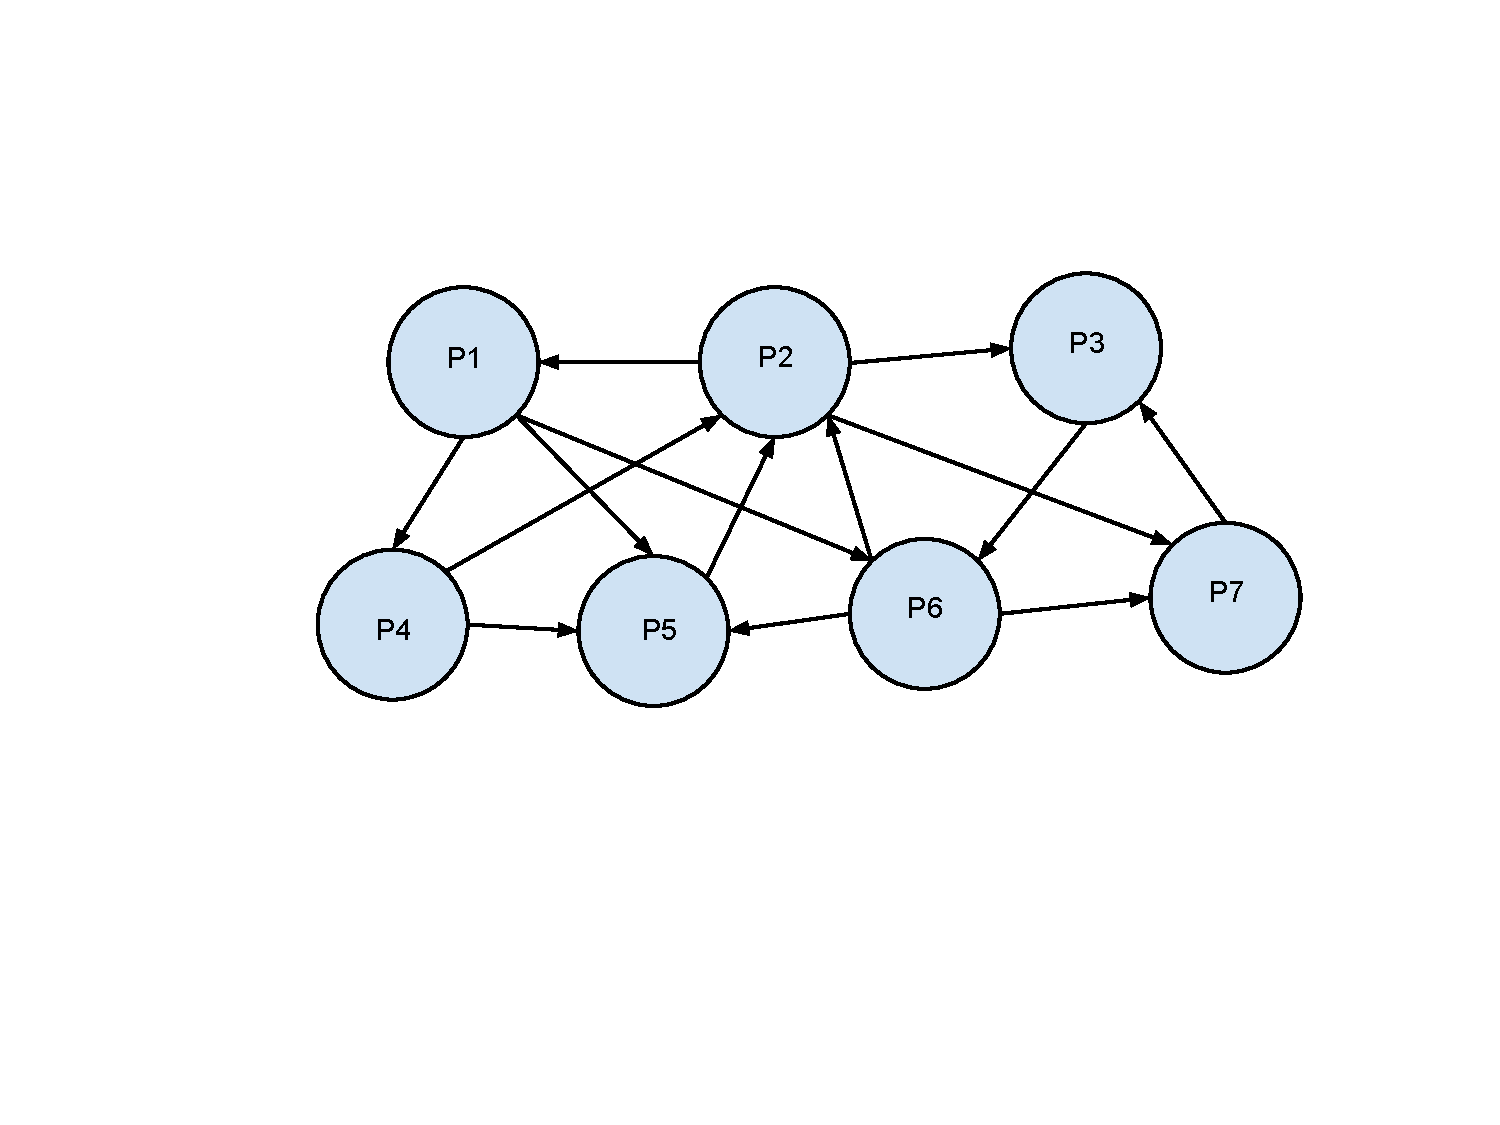
\includegraphics
[trim=40mm 50mm 4mm 20mm, clip, width=80mm]
{shuffle-graph.pdf}
\caption{
Data shuffling graph}
\label{fig:shuffle-graph}
\end{center}
\end{figure}


As shown in Figure \ref{fig:shuffle-graph}, each node is denoted as a process, which holds several data segments to move. A edge  represents the data shuffling direction and size. Note our data shuffling graph is a non-disparite graph.
Our goal here is to schedule all the data movements such that the overall completion time is minimized.

Our data shuffling problem can be considered as one variation of the   job shop scheduling problem, in which ideal jobs are assigned to resources at particular times\cite{garey1976complexity}. The job shop scheduling problem is well studied and knows as a NP-Hard problem \cite{adams1988shifting}. 
However, previous approximation methods can not be directly applied to our shuffling problem, as we have a very special constraint. In our setting, each process can either send or receive   data   at one time. When   process  A is sending data to process B, A and B need to collaborate  together to  finish this data transferring procedure.
Hence, there is a partially sequential dependence in the scheduling.
Each process has some data packages to send and also needs to receive some packages. We need to determine the order of data shuffling jobs for each process. We assume there is no cost for job transition. Our algorithm is based on the ideal case where the data transferring time is only based on the data size. 


 Two observations motivate our algorithm design. First,  the final completion time is determined by finishing scheduling all the data shuffling, especially those process with heavy workload. 
Thus, processes with heavy workload should have higher priority. Second, the more data is shuffled in parallel, the higher throughput we can obtain. Based on these two observations, we a multi-stage max-weight match finding (M3F) algorithm. For each process (node in our graph), we denote its workload as all data that it needs to receive and send. Then we define the weight of each edge (data shuffling request) as the sum of  workloads of sender node and receiver node. Note this weight is different from the original edge weight, which is the data size. The main idea of our algorithm is to iteratively find a max-weight near optimal match within our graph, and schedule all edges each match at one time. The edge weights are updated after each iteration. The iteration continues until all edges are scheduled. The pseudo code our our M3F algorithm is listed in Algorithm \ref{alg:m3f}.


\begin{algorithm}
\caption{Multi-stage max-weight match finding (M3F) algorithm}
\label{alg:m3f}
\begin{algorithmic}[1]
\STATE Initialize the non-scheduled edge set $S = \{\mbox{all edges}\}$ 
\REPEAT 
\STATE Initialize all nodes as idle
\REPEAT
\STATE Find an idle edge $e  \in S$ with largest weight in $S$
\STATE Mark nodes incident to $e$ as busy, and update their workload 
\STATE Delete $e$ from $S$
\UNTIL{No idle edge  can be scheduled } 
\UNTIL{$S$ is empty}
\end{algorithmic}
\end{algorithm}

Another   possibility is to all the jobs in a dynamic/online  manner. Instead of providing a static schedule of each job, we assign a greedy policy for each process. 
Each process holds a data transfer (send/receive) job list, and hence its overall workload can be computed. Further, each process also has a list 
of peers, for which the process needs to communicate data with. We sort this peer list based on each peer's workload.
Then each process performs a hand-shake communication with each peer, according to the sorted order.
If a peer is available, the process sets up the channel with the peer and transfer data. Otherwise, the process continues to hand-shake with the next peer, until finding an available one.
Each process repeat such processes until all jobs are finished.

We note our global algorithm is not global optimal. The time complexity of our algorithm is $O(n^2)$, with $n$ equals to the number of edges.  Our experimental evaluation shows our algorithm consistently outperforms a stochastic scheduling baseline.




%%%%%%%%%%%%%%%%%%%%%%%%%%%%
%%%%%%%%%%%%%%%%%%%%%%%%%%%%
%%%%%%%%%%%%%%%%%%%%%%%%%%%%
%%%%%%%%%%%%%%%%%%%%%%%%%%%%
\section{Implementation}
\label{sec:implementation}

\begin{figure}[ht]
    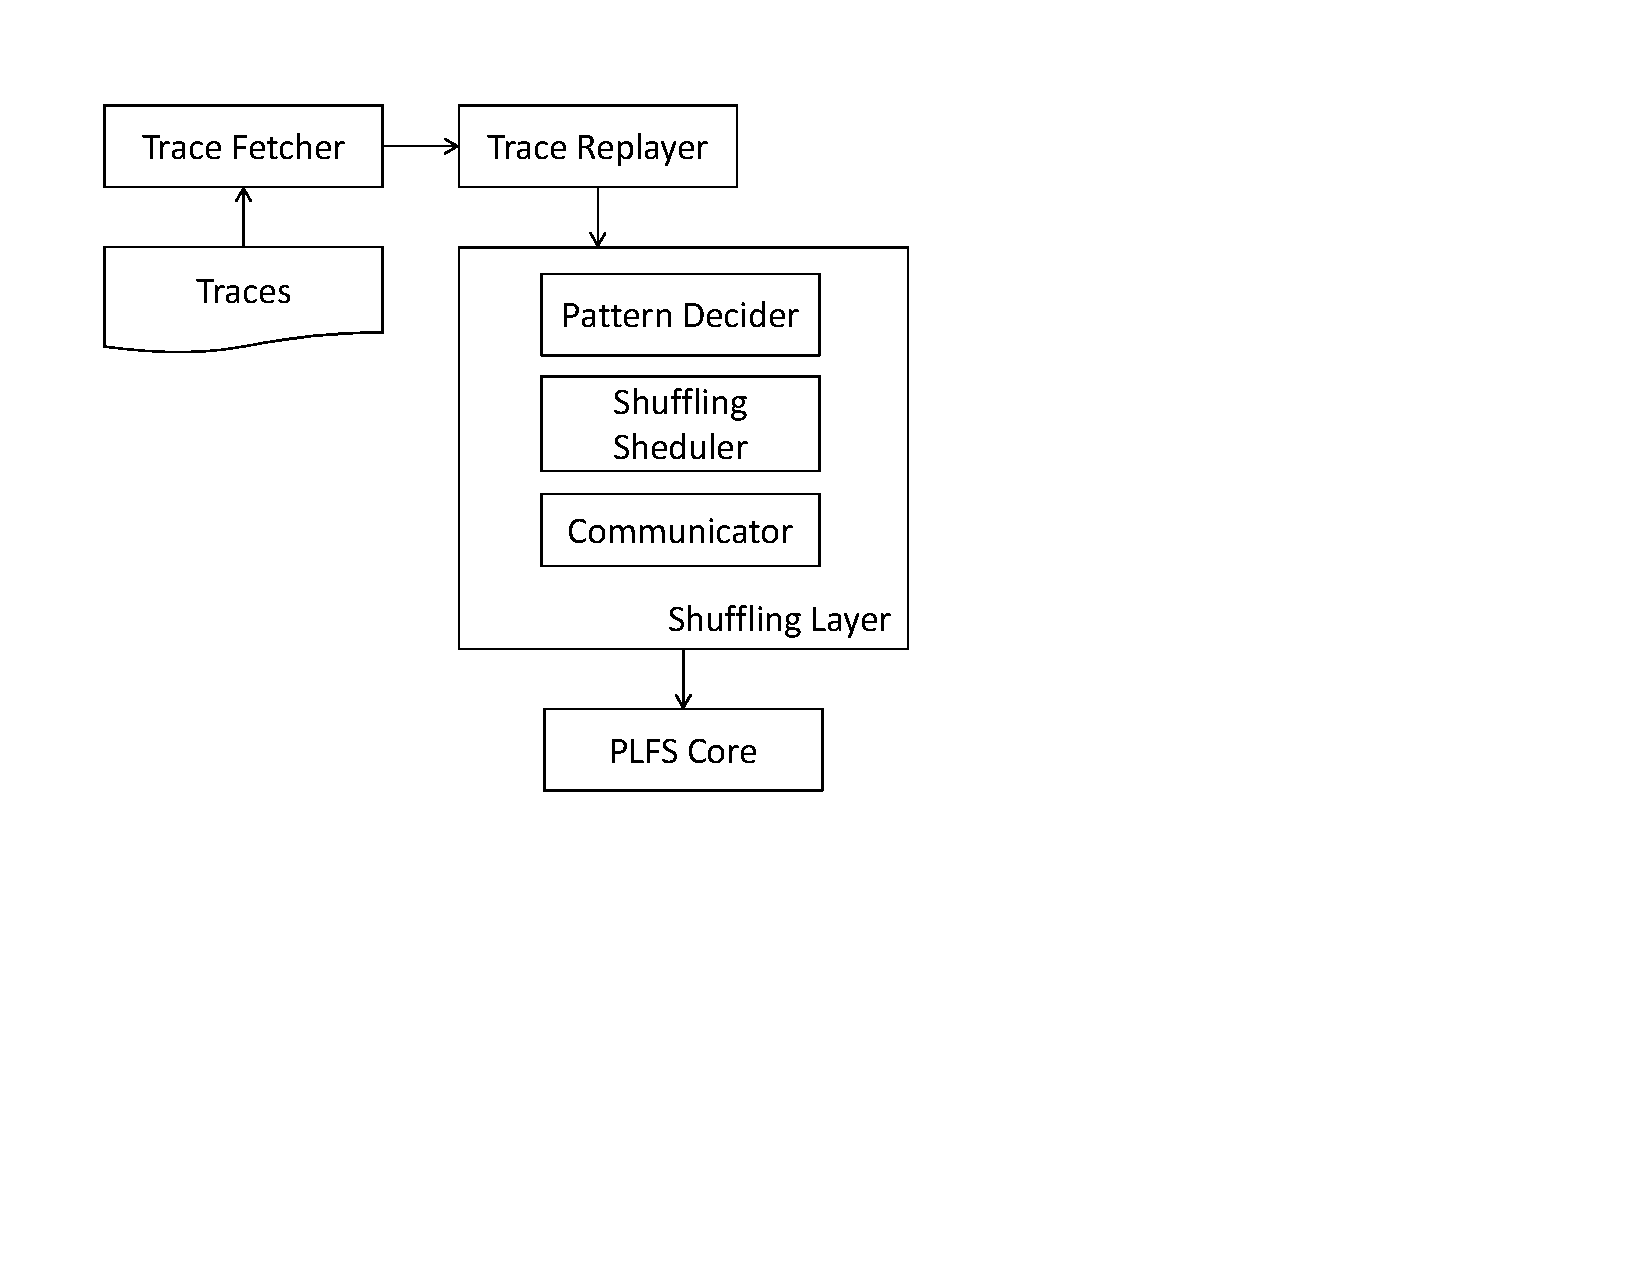
\includegraphics
    	[trim=0mm 80mm 120mm 0mm, clip, width=80mm]
    	{framework}
    \caption{System design}
    \label{fig:framework}
\end{figure}

Figure~\ref{fig:framework} shows the framework
of the system. Previously, many application
write traces are collected and available online\cite{plfsmap}.
The traces have pid, offset, length, indicating
which process writes to which part of the file.
To use these traces, we build a trace fetcher
to read the traces and sent them to
replayer processes. The replayer processes
do what is described in the traces. For example,
if there are four processes in the trace,
there will be four processes spawned by MPI.
Each process will do the job assigned to it.

The writes from the trace replayer will
reach the shuffling layer. The shuffling
layer buffers the data. It then collects
all the writes from all the processes
to a master process. The master process
uses the pattern decider (section~\ref{sec:creating-pattern})
to find a target pattern we want to create.
The pattern decider will also compare
the current writes and the target writes
to figure out what data should be moved.
This information is represented as a graph.
Later, the graph is passed to shuffling
scheduler. The scheduler will do
order the data movement activities.
Currently, there are two scheduling
algorithms - random and M3F. The output
of the scheduler will also be a graph,
but each edge has been assigned with
a order number. 

The scheduler graph is passed to the communicator.
The communicator distributes the edge
only to its associated processes. After
receiving all the edges, the process
will sort the edges by their order number
and do the operation indicated by the edges
one by one. After all the operations are done,
we write the shuffled data to PLFS core. 



%%%%%%%%%%%%%%%%%%%%%%%%%%%%
%%%%%%%%%%%%%%%%%%%%%%%%%%%%
%%%%%%%%%%%%%%%%%%%%%%%%%%%%
%%%%%%%%%%%%%%%%%%%%%%%%%%%%
\section{Evaluation}
\label{sec:evaluation}
\subsection{Setup}
The experiments are conducted at 
cluster with 64 nodes.
Each node is with 8 cores and 16GB RAM.
The operating system on the nodes
is Linux with kernel 2.6.32.
The communication between
processes is by OpenMPI 1.4.

\subsection{Log size compression}
To see how much the data shuffling
can reduce the log size, we investigated
traces of two applications - LANL app2
and Chombo. 

LANL app2 is an application with 
regular write pattern for the whole
file but the middle part of the file.
Since we only care about how much
we can compress the irregular write
log by shuffling data, we trimmed off
the parts that have regular patterns.
That means the trace fetcher only
fetches the irregular writes and
feeds them to the replayer. 

Chombo is an application with no
obvious patterns at all. We visualized
the writes to a chombo file
and found several groups of writes.
These writes are clustered at
certain parts of the file, but they
are irregular. We guess that
is because there are several `master'
processes holding a write job queue.
Other processes fetch jobs from the
queue after they finish their previous job.
In this way, which process gets to write
what data depends how fast they finish
the jobs.

Although deciding a good pattern is hard,
shuffling the data to compress
the log will always work. Figure~\ref{fig:logcompression}
shows the compression rates of three
cases - chombo with 128 proc, chombo with 64 proc,
LANL app2 with 128 proc. For all these
cases, the final log size will always be
about 100 bytes, thanks to data shuffling. 
Final log contains only one \emph{pattern} entry
instead of one entry for one write.
The compression rate is higher when the number
of writes is higher. Because no matter how
many writes the application has, there will
be only one final pattern entry. In the 
case of Figure~\ref{fig:logcompression},
chombo-128proc has the most writes.
So it has the highest compression rate. 
Note that we did not run the test on Pattern PLFS,
this is done theoretically. However,
based on our knowledge, we believe this will be the case.

\begin{figure}[ht]
    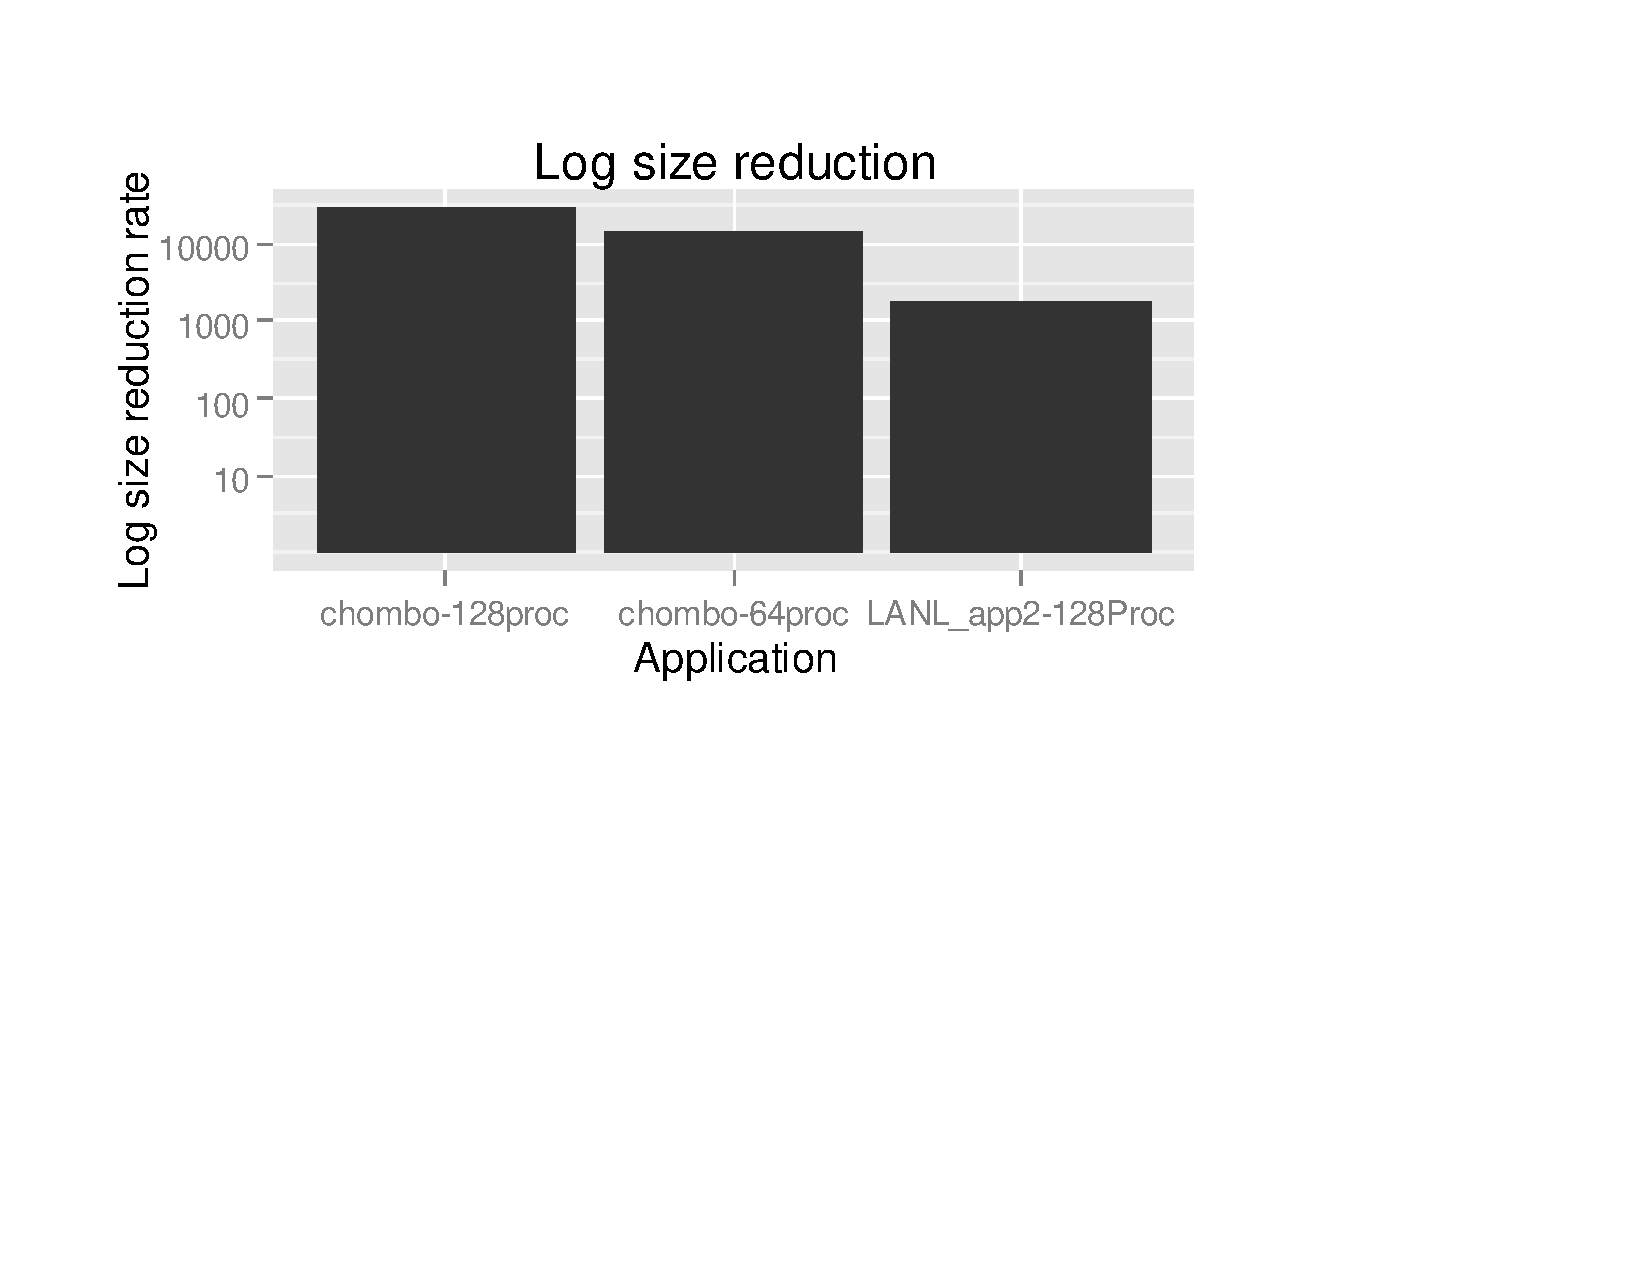
\includegraphics
    	[trim=20mm 90mm 80mm 0mm, clip, width=85mm]
    	{logcompression}
    \caption{Log compression rates}
    \label{fig:logcompression}
\end{figure}

\subsection{Shuffling bandwidth}
As we trade the data shuffling overhead
with the log size improvement,
we want to make sure that we can 
reduce the overhead as much as possible.
We try to do this by carefully scheduling
the data movement activities. 

\begin{figure}[ht]
    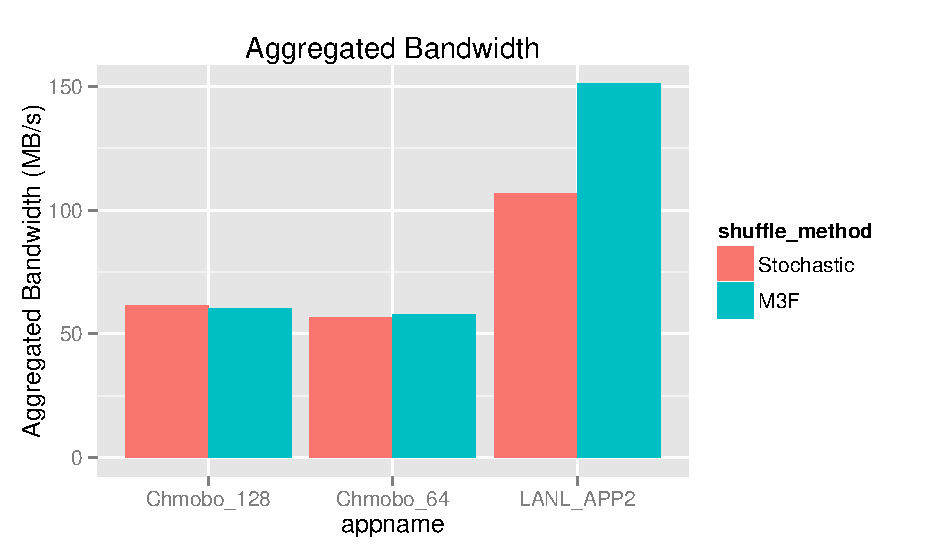
\includegraphics
    	[trim=0mm 0mm 10mm 0mm, clip, width=80mm]
    	{bw}
    \caption{Data shuffling bandwidth}
    \label{fig:bw}
\end{figure}

Figure~\ref{fig:bw} shows that our proposed
algorithm is almost the same as the stochastic
algorithm. This might be because the random
solution is already close to optimal. Spending
time to carefully schedule it did not help. 
For the LANL app2 case, our proposed algorithm
does have about 50\% higher bandwidth. We plan 
to future investigate the reason why
random solution is close to what we propose.
Note that, due to the limitation of our prototype,
we did not use the whole trace for our test in the
chombo cases. For LANL app2, we used the traces
with irregular writes.

%%%%%%%%%%%%%%%%%%%%%%%%%%%%
%%%%%%%%%%%%%%%%%%%%%%%%%%%%
%%%%%%%%%%%%%%%%%%%%%%%%%%%%
%%%%%%%%%%%%%%%%%%%%%%%%%%%%
\section{Future work}
\label{sec:future-work}
Finding better patterns with techniques
from digital signal processing is an interesting
topic. A better pattern can dramatically
reduce the size of data we need
to move and make this data shuffling
idea more practical. 

We also plan to find a better shuffling
design. Right now, we have one master process
that collects all the write information of all
the processes running. This effectively
places a barrier in all the processes. We
might be able to remove this barrier by
removing the master and replace it with a
totally distributed approach.


%%%%%%%%%%%%%%%%%%%%%%%%%%%%
%%%%%%%%%%%%%%%%%%%%%%%%%%%%
%%%%%%%%%%%%%%%%%%%%%%%%%%%%
%%%%%%%%%%%%%%%%%%%%%%%%%%%%
\section{Conclusions}
\label{sec:conclusions}
In this project, we investigate
the limitation of PLFS - its log.
We propose to solve the problem
by shuffling data between
distributed processes to create 
regular write patterns, so that
the pattern log compression feature
of PLFS can be enabled. 

This approach can significantly
reduce the log size and thus remove
the limitation of PLFS. The cost
of the shuffling data is reduced
by carefully scheduling the data movement
activities. We propose a scheduling
algorithm called M3F. We show
that it can increase the bandwidth
for an important application by about 50\%.


\bibliographystyle{abbrv}
\bibliography{report}  
\end{document}
